\documentclass[12pt,a4paper,titlepage]{report}

\usepackage[titletoc]{appendix}
\usepackage[nottoc]{tocbibind}
\usepackage{fancyhdr}
\usepackage{graphicx}
\usepackage[left=3.5cm, right=2.5cm, top=3.0cm, bottom=2.5cm]{geometry}
\usepackage{latexsym}
\usepackage{epsfig}
\usepackage{rotating}
\usepackage{eufrak}
\usepackage{type1cm}
\usepackage{newsec}
\usepackage{titlesec}
\usepackage{float}
\usepackage{amsmath}
\usepackage{array}
\usepackage{booktabs}
\usepackage{longtable}
\usepackage{multirow}
\usepackage{url}
\usepackage{tikz}
\usepackage{xcolor}
\usepackage{listings}
\usepackage[hidelinks]{hyperref}
\usetikzlibrary{arrows.meta,positioning,fit,shapes.geometric,shapes.symbols}

\titleformat{\chapter}[display]
{\normalfont\Large\bfseries\centering}{\chaptertitlename\ \thechapter}{25pt}{\Large}

\newcommand{\ReportTitle}{FLUIDWORKS: REAL-TIME CFD VISUALIZATION PLATFORM}
\newcommand{\ReportTitleMixed}{FluidWorks: Real-Time CFD Visualization Platform}
\newcommand{\LegacyProductName}{AeroFlow}

\definecolor{codebg}{RGB}{247,248,250}
\definecolor{codeframe}{RGB}{210,214,220}
\definecolor{codeblue}{RGB}{22,90,180}
\definecolor{codegreen}{RGB}{20,120,80}
\definecolor{codegray}{RGB}{110,110,110}

\lstdefinestyle{fluidworksstyle}{
backgroundcolor=\color{codebg},
basicstyle=\ttfamily\scriptsize,
breaklines=true,
captionpos=b,
columns=fullflexible,
commentstyle=\color{codegreen},
frame=single,
framerule=0.3pt,
keepspaces=true,
rulecolor=\color{codeframe},
keywordstyle=\color{codeblue}\bfseries,
numbers=left,
numbersep=8pt,
numberstyle=\tiny\color{codegray},
showstringspaces=false,
tabsize=4
}

\lstset{style=fluidworksstyle}

\begin{document}
\hypersetup{pageanchor=false}
\emergencystretch=2em
\sloppy

\titlepage
\thispagestyle{empty}
\begin{center}
\Large \textbf{FLUIDWORKS: REAL-TIME CFD\\VISUALIZATION PLATFORM}\\[2cm]
\large \textit{The Mini Project report submitted in partial fulfillment of the
requirements for the award of the degree of}\\[1cm]
{\huge {$\mathfrak {Bachelor\; of\; Technology}$}}\\[.5cm]
\textit{in}\\[.5cm]
{\Large \bf \itshape{{Artificial Intelligence \& Machine Learning}}}\\[1cm]
\large \textit{by}
\vskip1.0cm
\large{Abhinav Manoj} (\small{Reg. No. MCE23AIM003})\\
\large{Niranjan J} (\small{Reg. No. MCE23AIM047})\\
\large{Abhiram Vijaykumar Kaimal} (\small{Reg. No. MCE23AIM004})\\
\large{Rohan Tom Reji} (\small{Reg. No. MCE23AIM052})\\
\vskip1.0cm
\includegraphics[height=5cm]{college_logo-removebg.png}\\
\vspace{1cm}
\large \bfseries{Marian Engineering College}\\
\large \bfseries{Trivandrum}\\
\large \bfseries{Kerala}\\
\vspace{2cm}
\large \bfseries{March 2026}\\
\end{center}

\clearpage
\newlength{\toptafiddle}
\newlength{\bottafiddle}
\setlength{\toptafiddle}{1in}
\setlength{\bottafiddle}{1in}
\vspace*{-0.5in}
\enlargethispage{\bottafiddle}
\thispagestyle{empty}

\begin{center}
\Large \bfseries{DEPARTMENT OF ARTIFICIAL INTELLIGENCE \& MACHINE LEARNING}\\
\large\bfseries{Marian Engineering College}\\
\large \bfseries{Kazhakuttom, Trivandrum - 695582}\\
\vspace{1.0cm}
\includegraphics[height=6.0cm]{college_logo-removebg.png}\\
\vspace{1.5cm}
\textbf{CERTIFICATE}
\end{center}
\vspace{1.5cm}
\small This is to certify that the report entitled \textbf{``\ReportTitleMixed''} is a bonafide record
of the Mini Project presented by Abhinav Manoj (Reg. No. MCE23AIM003), Niranjan J (Reg. No. MCE23AIM047),
Abhiram Vijaykumar Kaimal (Reg. No. MCE23AIM004) and Rohan Tom Reji (Reg. No. MCE23AIM052) under our
supervision and guidance. The report has been submitted to the Department of Artificial Intelligence \& Machine Learning of Marian Engineering College, Kazhakuttom, Trivandrum in partial fulfillment of the award of the Degree of Bachelor of Technology in Artificial Intelligence \& Machine Learning, during the year 2025-2026.\\[.5cm]
\normalsize
\begin{center}
\line(1,0){425}
\end{center}
\vspace{1cm}
\begin{minipage}[t]{0.48\textwidth}
\begin{flushleft}
\textbf{Dr. Aswathy S U}\\
\itshape{Supervising Guide}\\
\itshape{Assistant Professor}\\
\itshape{Artificial Intelligence \& \\ Machine Learning}\\
\itshape{Marian Engineering College \\ Trivandrum}\\
\end{flushleft}
\end{minipage}
\hfill
\begin{minipage}[t]{0.48\textwidth}
\begin{flushleft}
\textbf{Prof. Balu John}\\
\itshape{Head of the Department}\\
\itshape{Artificial Intelligence \& \\ Machine Learning}\\
\itshape{Marian Engineering College \\ Trivandrum}\\
\end{flushleft}
\end{minipage}

\clearpage
\normalsize{}
\thispagestyle{empty}
\renewcommand\abstractname{ACKNOWLEDGEMENT}
\begin{abstract}
\vspace{1.5cm}
We express our sincere gratitude to our Principal \textbf{Dr. Abdul Nizar M.}, to \textbf{Prof. Balu John}, Head of the Department of Artificial Intelligence \& Machine Learning, and to the faculty members who supported the completion of this work. We record our special thanks to our supervising guide \textbf{Dr. Aswathy S. U} for the steady review, practical suggestions, and academic guidance that shaped both the software and this report. We also acknowledge our classmates and friends for their feedback during testing and demonstration. The project demanded work across simulation logic, user-interface design, documentation, and validation, and their support made that process manageable.
\end{abstract}

\newpage
\renewcommand\abstractname{ABSTRACT}
\begin{abstract}
\vspace{1.5cm}
\ReportTitleMixed{} is a Unity-based desktop platform for interactive CFD-style visualization. The current implementation centers on a maintained external-aero wind-tunnel path supported by a GPU grid solver, streamline and slice visualizations, vehicle-aware engineering estimates, runtime 3D model loading, and export-oriented reporting tools. The repository also includes an internal-flow workflow with explicit boundary assignment, surface pressure and friction views, rotating-machinery support, and free-surface experimentation. In addition to the simulation stack, the project contains a lightweight AI/ML-assisted geometry assessment layer that predicts aerodynamic tendencies from extracted shape features and presents actionable recommendations in the analysis interface. This report reorganizes the earlier FluidWorks documentation into the exact mini-project format required by the new reference template while preserving the established figures, tables, technical framing, and source-grounded explanations. The document covers background, system design, solver workflow, AI/ML components, testing strategy, observed outcomes, limitations, and representative appendix listings from the current repository.
\end{abstract}

\newpage
\pagenumbering{roman}
\normalsize \tableofcontents

\newpage
\normalsize \listoffigures

\newpage
\normalsize \listoftables

\newpage
\hypersetup{pageanchor=true}
\pagenumbering{arabic}
\setcounter{page}{1}

\pagestyle{fancy}
\setlength{\headheight}{15pt}
\fancyhead{}
\fancyfoot{}
\fancyhead[R]{\textit{\ReportTitleMixed}}
\fancyfoot[L]{\textit{Dept. of AI \& ML}}
\fancyfoot[R]{\textit{Marian Engineering College}}
\fancyfoot[C]{\thepage}
\renewcommand{\headrulewidth}{0.4pt}
\renewcommand{\footrulewidth}{0.4pt}

\chapter{Introduction}
\section{Overview}
FluidWorks is a real-time CFD-style visualization application built in Unity for fast engineering interpretation. The project does not target certification-grade numerical fidelity. Its purpose is different and more practical for a mini-project setting: load geometry quickly, configure a scenario with minimal friction, obtain readable flow visuals, and support the result with diagnostics that a reviewer can understand without stepping through a full industrial CFD workflow.

The current repository is not a thin prototype. It contains an actively maintained external-aerodynamics path, a dedicated internal-flow path, scene-level workflow selection, solver-side diagnostics, multiple visualization modes, export support, and a set of UI panels that expose the simulation in a structured way. The older product name \LegacyProductName{} still appears in namespaces and some file identifiers, but the present project identity is \textbf{FluidWorks}, and this report reflects the current state of that codebase.

\section{Motivation}
Traditional CFD packages are powerful, but they are often heavy in three ways: setup time, computational cost, and interpretation effort. Even before the first result appears, the user may have to prepare the mesh, assign boundaries carefully, choose solver models, monitor convergence, and post-process the output. That workflow is appropriate for detailed engineering studies, but it is not ideal for quick classroom demonstrations, early-stage concept reviews, or interactive exploration of imported geometry.

FluidWorks was motivated by that gap. The goal was to build a system that remains technically grounded while still feeling immediate. A user should be able to import a model, select a relevant simulation template, inspect the resulting field visually, and relate those visuals to values such as drag force, pressure drop, wall shear, divergence, or predicted aerodynamic quality. In short, the software should shorten the distance between ``load model'' and ``understand what is happening.''

\section{Problem Definition}
The central engineering problem addressed in this project can be expressed as follows:

\textit{How can a desktop application provide visually meaningful and technically defensible fluid-flow analysis across multiple engineering scenarios while remaining responsive enough for interactive use on commodity hardware?}

This problem is not solved by simply showing particles or by simply implementing equations. The project must connect geometry import, solver execution, boundary handling, user controls, visualization, diagnostics, and output generation. If any one of those layers is weak, the application stops being useful as a complete engineering tool.

\section{Objectives}
The present implementation is aimed at the following objectives:
\begin{enumerate}
\item build a single desktop interface that can host multiple flow-analysis workflows;
\item support runtime import of engineering geometry so that the same application can evaluate different models without recompilation;
\item provide a GPU-accelerated external-aero wind-tunnel path that stays visually stable during interaction;
\item provide an internal-flow path with explicit opening detection and boundary assignment;
\item expose diagnostics that support the visuals instead of leaving them as decorative output;
\item include an AI/ML-assisted geometry assessment layer for rapid model-quality feedback;
\item support capture and export of results in a report-friendly form; and
\item maintain a modular implementation that can be extended in future iterations.
\end{enumerate}

\section{Scope of the Project}
The project scope covers interactive external aero, internal flow, rotating-machinery visualization, and free-surface experimentation. Among these, the wind-tunnel path is the most mature and acts as the baseline solver workflow in the repository. The internal-flow path extends the software beyond vehicle-style demonstrations and introduces boundary-assignment logic, surface pressure view, and friction-oriented interpretation. The rotating-machinery and free-surface paths broaden the template catalog and show that the architecture can support more than one simulation family.

The scope does not include industrial turbulence-model depth, mesh-quality optimization pipelines, or certification-quality validation against standard benchmark datasets. Those areas would require much more numerical and hardware investment than is reasonable for this project. The emphasis here is educational usefulness, interactive response, and technically sensible behavior.

\section{Chapter Details}
This report is organized to match the mini-project reference format while retaining the engineering depth of the earlier FluidWorks report. Chapter 2 summarizes the technical background that motivated the project design. Chapter 3 explains the proposed system architecture and workflow. Chapter 4 discusses the tools and technologies used in the implementation. Chapter 5 presents the active simulation stacks in the repository. Chapter 6 describes the AI/ML components that are actually included in the project. Chapter 7 records testing strategy and observed results. Chapter 8 discusses applications, limitations, and future scope. Chapter 9 concludes the report, and the appendices provide representative listings from the current codebase.

\chapter{Literature Survey and Technical Background}
\section{Interactive CFD as an Engineering Need}
Computational Fluid Dynamics is usually introduced through the Navier-Stokes equations, discretization methods, and boundary-value problems \cite{anderson,versteeg,ferziger}. In practice, however, users encounter CFD through tools and workflows. For students and early-stage designers, the challenge is rarely the existence of equations alone. The challenge is the length of the route from geometry to insight. An interactive CFD-style platform shortens that route by reducing setup friction and emphasizing readable outputs.

This idea is increasingly relevant in education. Students understand pressure recovery, wake formation, blockage, and separation more quickly when they can change geometry or inlet settings and immediately see the result. The same is true for internal flow: pressure drop and wall-shear ideas become more concrete when the visualization and diagnostics move together.

\section{GPU-Oriented Simulation in a Teaching Context}
GPU compute is a natural choice for a project that values responsiveness. Structured grids, buffer-based updates, and repeated kernel execution map well to compute shaders \cite{harris,stam}. Even when the solver is simplified relative to a high-end CFD suite, the ability to update a field repeatedly on the GPU provides enough speed for interactive exploration.

In a mini-project context this matters for two reasons. First, it keeps the project technically ambitious by moving the heavy iterative work away from the CPU. Second, it lets visualization remain coupled to the solver instead of turning into an offline post-processing step. That coupling is a major reason why FluidWorks feels like a tool rather than a static demonstration.

\section{Visualization as a Core Engineering Layer}
Many student projects treat visualization as an afterthought. FluidWorks treats it as a primary engineering layer. Streamlines, slices, particles, and surface contours are not merely aesthetic additions; they are the main mechanism by which the user interprets the field. A clean diagnostic number can tell the user that drag has changed, but the visualization tells the user \textit{why} the change likely happened. That is especially important when the software is used for review, explanation, and comparison.

\section{Geometry-Aware Evaluation}
Another important background idea is that not every useful assessment needs a full flow solve. Some engineering judgments can be approximated from geometry itself. If a model is very blocky, highly asymmetric, rough, or poorly tapered, the software can flag that early. FluidWorks uses this idea in its AI/ML-assisted model-quality analysis. The system extracts interpretable geometric features and feeds them to a small neural predictor that estimates trends such as drag tendency, separation risk, downforce potential, and overall efficiency score \cite{bishop,goodfellow,molnar}.

\section{Educational Relevance}
The project is academically useful because it sits at the intersection of several areas commonly taught separately:
\begin{enumerate}
\item fluid mechanics, through drag, lift, pressure, vorticity, wall shear, and pressure drop;
\item numerical methods, through discretized solver updates and divergence control;
\item computer graphics, through scene-space rendering and compute-shader execution;
\item software engineering, through modular runtime architecture and export workflows; and
\item artificial intelligence, through lightweight predictive assessment and geometry-driven recommendations.
\end{enumerate}

\section{Difference from Conventional CFD Packages}
FluidWorks does not attempt to replace commercial or research CFD packages. It intentionally trades some numerical sophistication for interactivity, usability, and readability. The design assumptions are straightforward:
\begin{enumerate}
\item the user should obtain meaningful output quickly;
\item controls and diagnostics should remain in the same workspace;
\item the software should remain responsive on typical desktop hardware; and
\item the output should be suitable for explanation, demonstration, and report generation.
\end{enumerate}

Those assumptions define the project clearly and keep expectations realistic. The value of FluidWorks lies in the balance it strikes between technical grounding and usability.

\chapter{Proposed System}
\section{High-Level Architecture}
FluidWorks is organized as a layered runtime system. The user begins in the UI, chooses or loads a project, selects a workflow template, configures the scenario, and then interacts with a simulation driver that orchestrates the solver, diagnostics, and active visualizers.

\begin{figure}[H]
\centering
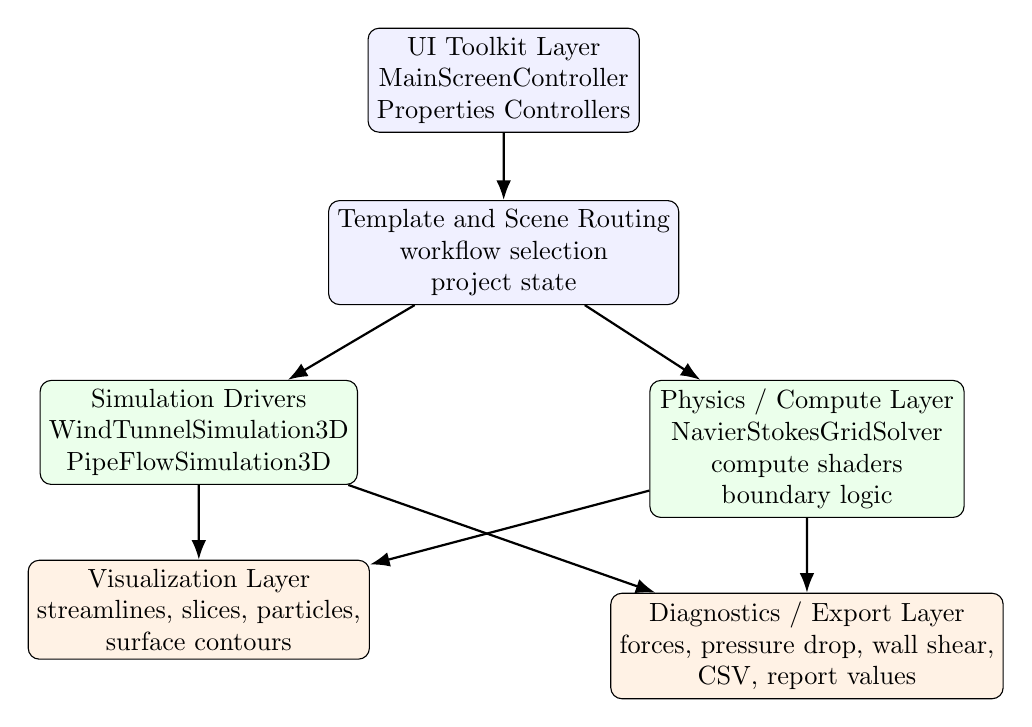
\begin{tikzpicture}[scale=0.95,transform shape,
node distance=0.9cm and 1.0cm,
box/.style={draw, rounded corners, align=center, minimum width=3.5cm, minimum height=0.95cm, fill=blue!6},
core/.style={draw, rounded corners, align=center, minimum width=4.2cm, minimum height=1.0cm, fill=green!8},
viz/.style={draw, rounded corners, align=center, minimum width=3.6cm, minimum height=0.95cm, fill=orange!10},
arrow/.style={-{Latex[length=2.5mm]}, thick}
]
\node[box] (ui) {UI Toolkit Layer\\MainScreenController\\Properties Controllers};
\node[box, below=of ui] (template) {Template and Scene Routing\\workflow selection\\project state};
\node[core, below left=1.0cm and -0.4cm of template] (sim) {Simulation Drivers\\WindTunnelSimulation3D\\PipeFlowSimulation3D};
\node[core, below right=1.0cm and -0.4cm of template] (solver) {Physics / Compute Layer\\NavierStokesGridSolver\\compute shaders\\boundary logic};
\node[viz, below=1.0cm of sim] (vis) {Visualization Layer\\streamlines, slices, particles,\\surface contours};
\node[viz, below=1.0cm of solver] (metrics) {Diagnostics / Export Layer\\forces, pressure drop, wall shear,\\CSV, report values};

\draw[arrow] (ui) -- (template);
\draw[arrow] (template) -- (sim);
\draw[arrow] (template) -- (solver);
\draw[arrow] (sim) -- (vis);
\draw[arrow] (solver) -- (vis);
\draw[arrow] (solver) -- (metrics);
\draw[arrow] (sim) -- (metrics);
\end{tikzpicture}
\caption{High-level architecture of the current FluidWorks runtime}
\label{fig:highlevel}
\end{figure}

\section{Implemented Workflow Summary}
\begin{table}[H]
\centering
\caption{Current simulation workflows in FluidWorks}
\label{tab:modes}
\begin{tabular}{p{3.0cm}p{4.2cm}p{6.3cm}}
\toprule
\textbf{Workflow} & \textbf{Primary Purpose} & \textbf{Current Notes} \\
\midrule
External Aero & Wind-tunnel style external flow around a vehicle or imported body & Most mature path; GPU Navier-Stokes grid solver, vehicle-aware outputs, multiple visualization contracts \\
Internal Flow & Pipe and duct style flow analysis & Mesh-driven boundary handling, opening classification, streamlines, and surface pressure / friction visualization \\
Rotating Machinery & Rotor, fan, propeller, and turbine style visualization & Runtime geometry workflow with rotating-region controls and machine-oriented diagnostics \\
Free Surface & Dam-break or splash-style study & GPU particle-style free-surface path for educational and demonstrative use \\
\bottomrule
\end{tabular}
\end{table}

\chapter{Simulation Workflows and Implementation}
\section{External Aero: Current Wind-Tunnel Stack}
The wind-tunnel path is the strongest implementation in the repository and acts as the baseline engineering workflow. \path{WindTunnelSimulation3D.cs} is the runtime driver. It owns initialization, playback, state validation, and solver orchestration. The repository guidance also makes it clear that the tunnel flow axis must remain explicit through \texttt{flowAxis}. The older longest-axis heuristic is not to be reintroduced because it produced ambiguous behavior in nonstandard tunnel shapes.

The active solver path uses \path{NavierStokesGridSolver.cs} together with the compute shader \path{NavierStokes3D.compute}. This pair handles field stepping, obstacle coupling, pressure-related correction, and diagnostics such as divergence and vorticity. Obstacle interaction depends on \path{ObstacleVoxelizer.cs} as well, which converts loaded geometry into a representation the solver can use.

\section{Wind-Tunnel Visualization Contract}
The visualization contract in the repository is explicit and worth documenting because it prevents mode confusion:
\begin{enumerate}
\item \textbf{Effects} is the stylized wake mode and is intended to give a readable impression of flow motion around a loaded vehicle.
\item \textbf{Velocity} uses compact solver-driven slices and focused streamlines.
\item \textbf{Pressure} combines model pressure visualization with a body-adjacent slice rather than a full-screen slab.
\item \textbf{Surface Pressure} remains a body-only contour mode and should not replace the broader pressure view.
\end{enumerate}

This contract matters because visualization quality can easily degrade when a project accumulates overlapping modes that appear similar. FluidWorks avoids that by giving each mode a clear purpose.

\begin{table}[H]
\centering
\caption{Wind-tunnel visualization expectations reflected in the repository}
\label{tab:windmodes}
\begin{tabular}{p{2.8cm}p{3.6cm}p{6.4cm}}
\toprule
\textbf{Mode} & \textbf{Primary Output} & \textbf{Expected Behavior} \\
\midrule
Effects & Stylized wake and motion impression & Readable body wake, not a raw diagnostic slab \\
Velocity & Streamlines and compact slices & Solver-driven views with focused interpretation \\
Pressure & Model pressure plus body-adjacent slice & Local pressure understanding without screen-filling clutter \\
Surface Pressure & Body-only contour & Additive contour mode separated from the broader pressure view \\
\bottomrule
\end{tabular}
\end{table}

\section{Streamline Rendering Quality}
The repository notes place unusual emphasis on streamline quality, and that is justified. A weak streamline presentation makes the solver look less credible even when the field is numerically stable. The current expectations are clear:
\begin{enumerate}
\item solver data remains the primary velocity source;
\item seed positions use a stable random sequence to avoid frame flicker;
\item lines must be long enough to traverse a meaningful portion of the tunnel;
\item wake regions must not be eliminated by an aggressive speed-kill threshold; and
\item the palette should remain vivid enough to communicate velocity changes.
\end{enumerate}

These details may sound cosmetic, but they are essential to the user experience. A user forms trust in the system largely through stable and interpretable output.

\section{Vehicle-Aware Engineering Outputs}
The wind-tunnel path also exposes derived estimates through the analysis interface. These include drag force, vertical aero force, downforce, center of pressure, pitch, yaw, and roll moments, axle loads, and estimated top speed. The repository guidance explicitly separates those values from solver diagnostics such as divergence error and mean vorticity. That separation is important because the first group is vehicle-oriented interpretation, whereas the second group is field-quality and solver-health feedback.

\section{Internal Flow: Updated Pipeline}
The internal-flow path extends the platform beyond vehicle-style studies. \path{PipeFlowSimulation3D.cs} manages the domain, solver stepping, and metric sampling for pipe and duct analysis. A significant recent improvement is the explicit role of \path{BoundaryConditionManager.cs}. Internal flow is much more sensitive to opening meaning than a simple wind tunnel, so the project now treats boundary assignment as a workflow requirement rather than an invisible assumption.

\section{Boundary Assignment and Surface Views}
The internal-flow workflow uses detected openings, user-assigned inlet and outlet semantics, and surface-driven diagnostics such as pressure and friction visualization. This is one of the strongest signs that the project has matured. Rather than presenting only a volume field, the software now gives the user a body-coupled interpretation of what the field is doing at the wall. For report preparation, this is especially valuable because surface views communicate more directly than abstract field slices.

\section{User Workflow}
In practical use, a typical FluidWorks session follows a predictable path: load or recover a model, choose the relevant template, configure settings, run the solver, inspect the active visual mode, and export a result package if needed.

\begin{figure}[H]
\centering
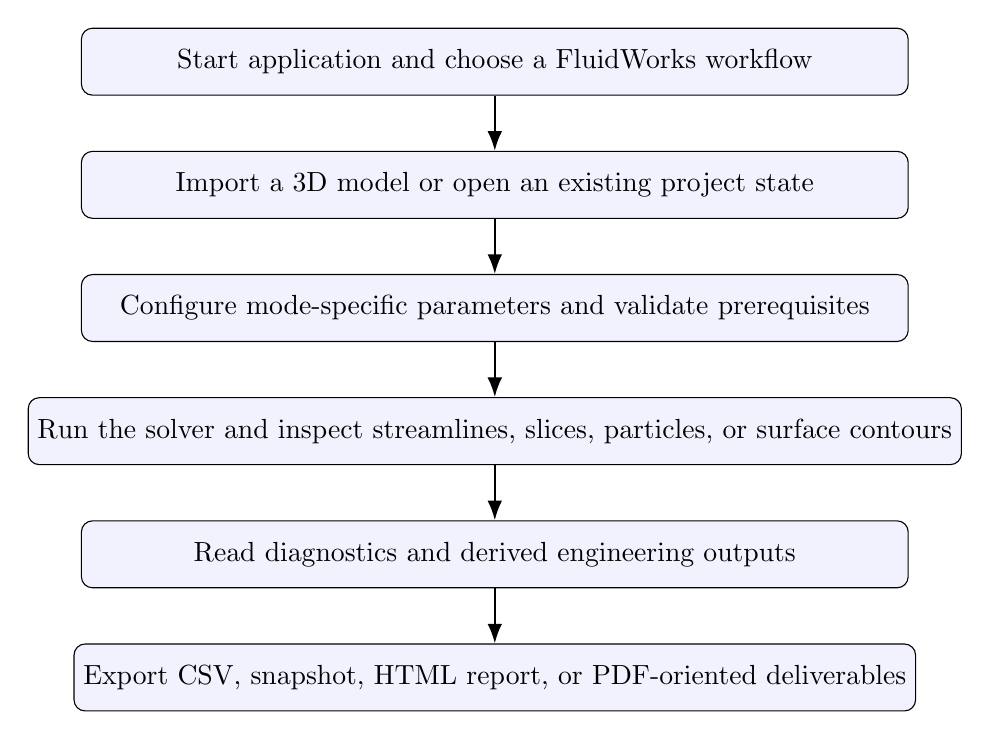
\begin{tikzpicture}[
node distance=0.7cm,
block/.style={draw, rounded corners, minimum width=10.5cm, minimum height=0.85cm, align=center, fill=blue!5},
arrow/.style={-{Latex[length=2.5mm]}, thick}
]
\node[block] (u1) {Start application and choose a FluidWorks workflow};
\node[block, below=of u1] (u2) {Import a 3D model or open an existing project state};
\node[block, below=of u2] (u3) {Configure mode-specific parameters and validate prerequisites};
\node[block, below=of u3] (u4) {Run the solver and inspect streamlines, slices, particles, or surface contours};
\node[block, below=of u4] (u5) {Read diagnostics and derived engineering outputs};
\node[block, below=of u5] (u6) {Export CSV, snapshot, HTML report, or PDF-oriented deliverables};
\draw[arrow] (u1) -- (u2);
\draw[arrow] (u2) -- (u3);
\draw[arrow] (u3) -- (u4);
\draw[arrow] (u4) -- (u5);
\draw[arrow] (u5) -- (u6);
\end{tikzpicture}
\caption{Typical user workflow in FluidWorks}
\label{fig:userworkflow}
\end{figure}

\section{Implementation Observations}
Two implementation choices stand out when the repository is read as a complete system. First, the project consistently favors explicit control over hidden heuristics. The explicit flow axis and explicit boundary assignment are both examples of this. Second, the project favors readable engineering output over excessively dense screens. The visualization contract, the solver diagnostics grouping, and the separation between model-quality assessment and field diagnostics all follow that principle.

\chapter{AI/ML Components Included in the Project}
\section{Why AI/ML Was Included}
The project belongs to the Artificial Intelligence \& Machine Learning domain, so the final report should document where AI/ML is genuinely used. In FluidWorks, AI/ML does not replace the CFD-style solver. Instead, it complements the simulation with a fast geometry-aware assessment layer. This is a sensible design choice because some questions can be answered directly from shape features long before a user studies the full flow field in detail.

\section{Aero Geometry Analysis Pipeline}
The AI/ML functionality is centered on two repository files: \path{AeroGeometryAnalyzer.cs} and \path{AeroMLPredictor.cs}. The first file extracts geometric descriptors from the currently loaded model. The second file applies a lightweight neural network to those descriptors and returns a set of predictive values.

The extracted feature set is deliberately interpretable. It includes aspect ratio, slenderness ratio, frontal blockage ratio, volume efficiency, surface roughness, symmetry score, underside clearance, and rear taper ratio. These are not arbitrary neural inputs. They are quantities with direct aerodynamic meaning, which makes the resulting analysis easier to explain during evaluation.

\section{ML Predictor Design}
The predictor itself is implemented as a small multilayer perceptron with fixed, physics-informed weights. According to the source file comments, the network architecture is:
\begin{enumerate}
\item 8 input features;
\item 16 neurons in the first hidden layer with ReLU activation;
\item 8 neurons in the second hidden layer with ReLU activation; and
\item 4 output values passed through a sigmoid-scaled interpretation layer.
\end{enumerate}

The output values are:
\begin{enumerate}
\item predicted drag-coefficient tendency;
\item separation-risk estimate;
\item downforce-potential estimate; and
\item overall efficiency score.
\end{enumerate}

This is a sensible design for the project because it keeps inference local, dependency-free, and fast. The implementation does not depend on an external runtime such as ONNX or TensorFlow. That keeps deployment simple and avoids turning the ML component into a separate infrastructure problem. The design also matches the educational value of compact feed-forward models discussed in standard machine-learning texts \cite{bishop,goodfellow}.

\section{Feature Importance and Explainability}
One of the strongest AI/ML-related decisions in the repository is the inclusion of feature-importance estimation. The predictor computes central-difference sensitivity by perturbing each input feature and aggregating output variation. This is valuable for two reasons. First, it prevents the ML result from appearing as an unexplained black-box label. Second, it lets the software convert feature sensitivity into readable breakdown text and improvement suggestions. In that sense the project follows the broader direction of interpretable or explainable ML, where a model should assist human judgment rather than replace it blindly \cite{molnar,ribeiro}.

In practical terms, the user is not shown only a score. The software can report that blockage, roughness, taper, or symmetry had a high influence on the assessment. That makes the AI/ML layer much more appropriate for an academic project because the reasoning remains inspectable.

\section{Improvement Suggestions}
The geometry analyzer converts feature values and ML outputs into ranked design suggestions. The logic in the repository checks for high roughness, high blockage, weak rear taper, low aspect ratio, poor symmetry, very low clearance, and low volume efficiency. It also adds direct warnings when the model predicts high separation risk or high drag tendency. This turns the AI/ML output into something actionable instead of merely descriptive.

\section{Analysis Interface Integration}
The AI/ML outputs are not hidden in code. The analysis interface contains a dedicated ``Model Quality Analysis (ML)'' group. The UI labels display:
\begin{enumerate}
\item overall model quality score;
\item grade;
\item predicted drag-coefficient range;
\item separation risk;
\item downforce potential;
\item ML efficiency score;
\item geometric feature breakdown; and
\item improvement suggestions.
\end{enumerate}

This is important because it shows that the ML component is a user-facing product feature, not just a silent experiment inside the repository.

\section{Auto Segmentation Workflow}
The project also includes an ``Auto Segment Model'' action in the segmentation interface. This does not function as a large standalone ML system, but it is part of the broader intelligent-assistance story in the application. The segmentation controller can trigger automatic splitting and auto-identification of parts when the imported model needs motion-aware classification. In a workflow that supports rotating machinery and moving parts, this reduces manual setup effort and improves usability.

\section{AI/ML Workflow Summary}
\begin{figure}[H]
\centering
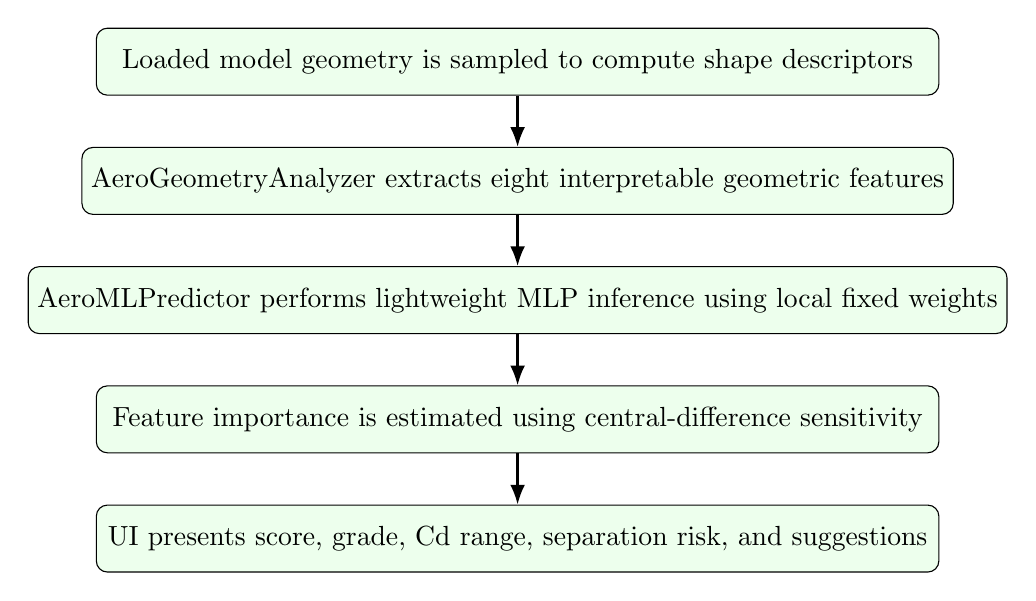
\begin{tikzpicture}[
node distance=0.65cm,
block/.style={draw, rounded corners, minimum width=10.7cm, minimum height=0.85cm, align=center, fill=green!7},
arrow/.style={-{Latex[length=2.5mm]}, thick}
]
\node[block] (m1) {Loaded model geometry is sampled to compute shape descriptors};
\node[block, below=of m1] (m2) {AeroGeometryAnalyzer extracts eight interpretable geometric features};
\node[block, below=of m2] (m3) {AeroMLPredictor performs lightweight MLP inference using local fixed weights};
\node[block, below=of m3] (m4) {Feature importance is estimated using central-difference sensitivity};
\node[block, below=of m4] (m5) {UI presents score, grade, Cd range, separation risk, and suggestions};
\draw[arrow] (m1) -- (m2);
\draw[arrow] (m2) -- (m3);
\draw[arrow] (m3) -- (m4);
\draw[arrow] (m4) -- (m5);
\end{tikzpicture}
\caption{AI/ML-assisted model quality workflow in FluidWorks}
\label{fig:mlflow}
\end{figure}

\section{Value and Limitations of the AI/ML Layer}
The AI/ML component adds clear value because it gives immediate design feedback even before the user spends time interpreting the full simulation result. It also aligns the project more closely with the degree program by introducing a predictive layer that is fast, explainable, and integrated into the main product workflow.

At the same time, its limitations should be stated plainly. The model is lightweight, physics-informed, and hand-embedded into the application. It is not trained online, it does not replace the solver, and it should be understood as an assistive estimator. In the context of this project, that is the correct scope. The strength of the feature is that it improves interaction and interpretation without pretending to be more than it is.

\chapter{Testing Strategies \& Result Achieved}
\section{Validation Approach}
The repository guidance makes it clear that validation should focus on behavior, stability, and technical credibility. For the wind-tunnel path, that means verifying mode switching, readable solver diagnostics, explicit flow-direction handling, reasonable wake behavior, and stable visualization output. For internal flow, it means checking that openings are identified correctly, boundaries are assigned before analysis, and surface pressure or friction views remain consistent with the computed field.

\section{Compile and Build Discipline}
The project notes also require a Unity batch compile check after non-trivial changes and a Windows batch build after compile success. This is an important engineering habit because Unity-based projects can fail at script-compile stage, scene binding stage, or build-export stage even when individual scripts look correct in isolation.

\section{Representative Validation Targets}
\begin{table}[H]
\centering
\caption{Representative validation targets in the current repository}
\label{tab:validation}
\begin{tabular}{p{3.2cm}p{4.9cm}p{4.8cm}}
\toprule
\textbf{Workflow} & \textbf{What is checked} & \textbf{Expected outcome} \\
\midrule
External Aero & Mode switching, yaw response, custom wind direction, turbulence stress & Stable visuals, clear mode replacement, no screen-filling artifacts \\
External Aero & Solver diagnostics & Readable values for divergence error and mean vorticity \\
Internal Flow & Boundary assignment and opening detection & Valid inlet and outlet setup before analysis \\
Internal Flow & Pressure and friction contours & Surface feedback remains tied to computed field behavior \\
UI / Workflow & Template selection, property binding, export triggers & Controls map correctly to active simulation state \\
AI / ML & Geometry assessment labels and suggestions & Quality score, grade, feature breakdown, and recommendations update for loaded models \\
\bottomrule
\end{tabular}
\end{table}

\section{Results Interpretation}
The project outcome is best understood through the kind of insight it gives to the user.

For external aero, the user can inspect stagnation at the front of the model, acceleration along the body, wake formation at the rear, asymmetry under yaw, and the way those patterns relate to drag and load estimates. For internal flow, the user can inspect whether the fluid path remains continuous through a cavity, where pressure loss concentrates, and where wall interaction intensifies. The software does not merely state that something changed; it gives a visual narrative that explains why the change matters.

\section{Observed Strengths}
The strongest achieved results in the current repository are:
\begin{enumerate}
\item a mature wind-tunnel path with explicit design rules;
\item stable solver-oriented visual outputs that remain readable in presentation settings;
\item a stronger internal-flow workflow than the earlier report documented;
\item export-friendly metrics and report support; and
\item a meaningful AI/ML-assisted analysis layer instead of a purely symbolic AI mention.
\end{enumerate}

\section{Limitations}
The present build still has clear limitations:
\begin{enumerate}
\item it is not a replacement for high-fidelity commercial CFD software;
\item the quality of interpretation is stronger than the claim of absolute numerical precision;
\item high resolutions or unsuitable hardware can reduce performance;
\item some workflows remain less mature than the wind-tunnel baseline; and
\item the AI/ML predictor is intentionally lightweight and should be treated as assistive rather than authoritative.
\end{enumerate}

\section{Why the Revised Report Matters}
The earlier report was adequate as a summary, but it was too short for a full mini-project submission and too light on implementation evidence. This revised version is more appropriate for evaluation because it documents solver organization, workflow structure, visualization rules, AI/ML inclusion, and source-grounded implementation decisions in a format that matches the new reference template.

\chapter{Applications, Discussion and Future Enhancements}
\section{Practical Applications}
FluidWorks can be applied in several realistic contexts:
\begin{enumerate}
\item classroom demonstration of aerodynamic and internal-flow concepts;
\item rapid comparison of alternate body shapes or duct layouts;
\item visual support during mini-project reviews and viva discussions;
\item exploratory analysis before moving to heavier CFD packages; and
\item interactive proof-of-concept work for future engineering software.
\end{enumerate}

\section{Discussion}
One of the strongest aspects of the project is that it joins simulation, interpretation, and presentation into a single workflow. That is often where student engineering tools fall short. A project may solve something numerically but fail to communicate it well, or it may look attractive but fail to expose real metrics. FluidWorks is more balanced. It uses visualization as an engineering aid, not as decoration, and it anchors those visuals to diagnostics that can be explained during evaluation.

The AI/ML layer also improves the project in a practical way. Instead of adding a detached machine-learning experiment for the sake of the degree title, the repository embeds a predictor where it is useful: in early geometry assessment and model-quality explanation. That makes the AI/ML inclusion coherent with the rest of the software.

\section{Future Enhancements}
Several extensions would strengthen the platform further:
\begin{enumerate}
\item selectable solver presets with clearer trade-offs between speed and quality;
\item richer boundary and material models for internal flow;
\item comparative multi-model analysis inside one project session;
\item broader export formats and automated summary generation;
\item stronger benchmark-based validation against known reference cases; and
\item expansion of the AI/ML layer into setup recommendation or anomaly detection.
\end{enumerate}

\chapter{Conclusion \& Future Work}
FluidWorks has developed into a practical real-time CFD-style visualization platform with a clear architectural center: a maintained wind-tunnel workflow supported by GPU solving, runtime model handling, readable visualization modes, and engineering-focused diagnostics. The repository also shows meaningful progress in internal-flow analysis, especially through explicit boundary assignment and surface-based diagnostics.

The inclusion of AI/ML in the current project is also genuine and relevant. The lightweight geometry-analysis pipeline adds predictive feedback, feature sensitivity, and actionable design suggestions without disrupting the core solver workflow. This makes the software more useful during early exploration and better aligned with the academic domain of the degree program.

In its current state, FluidWorks should be understood as an interactive educational and concept-analysis platform. It sits between classroom theory and heavyweight offline CFD workflows. That position gives the project both technical value and practical usefulness, and it provides a credible foundation for future expansion in simulation quality, design intelligence, and automated engineering assistance.

\begin{thebibliography}{15}
\bibitem{anderson}
J. D. Anderson,
\textit{Computational Fluid Dynamics: The Basics with Applications}.
New York, NY, USA: McGraw-Hill, 1995.

\bibitem{versteeg}
H. K. Versteeg and W. Malalasekera,
\textit{An Introduction to Computational Fluid Dynamics: The Finite Volume Method}, 2nd ed.
Harlow, U.K.: Pearson, 2007.

\bibitem{white}
F. M. White,
\textit{Fluid Mechanics}, 8th ed.
New York, NY, USA: McGraw-Hill, 2016.

\bibitem{ferziger}
J. H. Ferziger and M. Peric,
\textit{Computational Methods for Fluid Dynamics}, 3rd ed.
Berlin, Germany: Springer, 2002.

\bibitem{bridson}
R. Bridson,
\textit{Fluid Simulation for Computer Graphics}, 2nd ed.
Boca Raton, FL, USA: CRC Press, 2015.

\bibitem{stam}
J. Stam, ``Stable fluids,'' in \textit{Proc. 26th Annu. Conf. Computer Graphics and Interactive Techniques (SIGGRAPH)}, 1999, pp. 121--128.

\bibitem{harris}
M. J. Harris, ``Fast fluid dynamics simulation on the GPU,'' in \textit{GPU Gems}, R. Fernando, Ed.
Boston, MA, USA: Addison-Wesley, 2004, ch. 38.

\bibitem{unity}
Unity Technologies,
\textit{Unity Manual and Compute Shader Documentation}. [Online]. Available:
\url{https://docs.unity3d.com/}.

\bibitem{bishop}
C. M. Bishop,
\textit{Pattern Recognition and Machine Learning}.
New York, NY, USA: Springer, 2006.

\bibitem{goodfellow}
I. Goodfellow, Y. Bengio, and A. Courville,
\textit{Deep Learning}.
Cambridge, MA, USA: MIT Press, 2016.

\bibitem{molnar}
C. Molnar,
\textit{Interpretable Machine Learning}, 2nd ed.
[Online]. Available: \url{https://christophm.github.io/interpretable-ml-book/}

\bibitem{ribeiro}
M. T. Ribeiro, S. Singh, and C. Guestrin, ``Why should I trust you?: Explaining the predictions of any classifier,'' in \textit{Proc. 22nd ACM SIGKDD Int. Conf. Knowledge Discovery and Data Mining}, 2016, pp. 1135--1144.

\bibitem{pope}
S. B. Pope,
\textit{Turbulent Flows}.
Cambridge, U.K.: Cambridge Univ. Press, 2000.

\bibitem{patankar}
S. V. Patankar,
\textit{Numerical Heat Transfer and Fluid Flow}.
Boca Raton, FL, USA: CRC Press, 1980.

\bibitem{tu}
J. Tu, G. H. Yeoh, and C. Liu,
\textit{Computational Fluid Dynamics: A Practical Approach}, 3rd ed.
Oxford, U.K.: Butterworth-Heinemann, 2023.
\end{thebibliography}

\begin{appendices}
\chapter{Wind-Tunnel Runtime Driver Excerpt}
This appendix provides the opening portion of the wind-tunnel runtime driver, which is the central orchestration point for the maintained external-aero workflow.

\lstinputlisting[language={[Sharp]C},firstline=1,lastline=340,caption={Excerpt from the wind-tunnel runtime driver},label={lst:winddriver}]{appendix_src/WindTunnelSimulation3D.cs}

\chapter{Navier-Stokes Grid Solver Excerpt}
The following excerpt grounds the report's discussion of solver-side grid handling, diagnostics, and obstacle coupling.

\lstinputlisting[language={[Sharp]C},firstline=1,lastline=300,caption={Excerpt from the grid solver implementation},label={lst:gridsolver}]{appendix_src/NavierStokesGridSolver.cs}

\chapter{Compute Shader Excerpt}
This listing shows a representative section of the compute-shader implementation used by the wind-tunnel solver path.

\lstinputlisting[language=C,firstline=1,lastline=220,caption={Excerpt from the wind-tunnel compute shader},label={lst:computeshader}]{appendix_src/NavierStokes3D.compute}

\chapter{AI/ML Predictor Excerpt}
This appendix captures the lightweight multilayer perceptron used for geometry-based aerodynamic prediction.

\lstinputlisting[language={[Sharp]C},firstline=1,lastline=188,caption={AeroMLPredictor implementation},label={lst:mlpredictor}]{appendix_src/AeroMLPredictor.cs}

\chapter{Geometry Analysis Excerpt}
The geometry-analysis excerpt shows how the project converts model shape into interpretable features and model-improvement suggestions.

\lstinputlisting[language={[Sharp]C},firstline=1,lastline=210,caption={Excerpt from the geometry analyzer},label={lst:geomanalyzer}]{appendix_src/AeroGeometryAnalyzer.cs}

\chapter{Project Save Manager Excerpt}
This short appendix documents the project persistence layer used to save and recover analysis state.

\lstinputlisting[language={[Sharp]C},firstline=1,lastline=89,caption={Project save manager implementation},label={lst:save}]{appendix_src/ProjectSaveManager.cs}

\chapter{Project Data Model Excerpt}
The data model excerpt shows how project metadata and saved simulation configuration are structured inside the application.

\lstinputlisting[language={[Sharp]C},firstline=1,lastline=73,caption={Project data model implementation},label={lst:projectdata}]{appendix_src/ProjectData.cs}

\end{appendices}

\end{document}

\section{Module Description}
The project can be understood through five major module groups.

\subsection{User Interface Layer}
The UI layer is responsible for workflow selection, mode-specific controls, metrics display, and export actions. Because the project supports multiple simulation families, the UI has to remain adaptive without becoming confusing. This is why the repository uses dedicated property controllers and a centralized main screen controller rather than a single monolithic panel.

\subsection{Simulation Drivers}
Each simulation family has a driver that understands its own setup rules. For the wind-tunnel mode this role is played by \texttt{WindTunnelSimulation3D}. For internal flow it is handled by \texttt{PipeFlowSimulation3D}. These drivers translate user settings into solver state, manage initialization, and coordinate when visualizers should update.

\subsection{Solver and Physics Layer}
The physics layer stores and updates the field representation. In the wind-tunnel path this includes obstacle voxelization, grid buffers, pressure correction, velocity stepping, and solver diagnostics. In the internal-flow path the same idea is extended with explicit opening classification and boundary-condition enforcement.

\subsection{Visualization Layer}
The visualization layer exists to make the field readable. Streamlines show path tendency, field slices reveal interior variation, particles highlight motion and wake development, and surface contours allow the user to relate results directly to the imported body.

\subsection{Diagnostics and Export Layer}
A simulation without interpretable output is not useful for an academic report. FluidWorks therefore includes diagnostics for drag, vertical aero force, center of pressure, axle loads, pressure drop, wall shear, divergence, and related values. Export logic then packages those values into CSV, JSON, HTML, and PDF-oriented workflows.

\section{Data Flow Through a Runtime Frame}
The runtime sequence can be described as a loop that begins with configuration state, passes through solver execution, and ends with visualization and diagnostics refresh.

\begin{figure}[H]
\centering
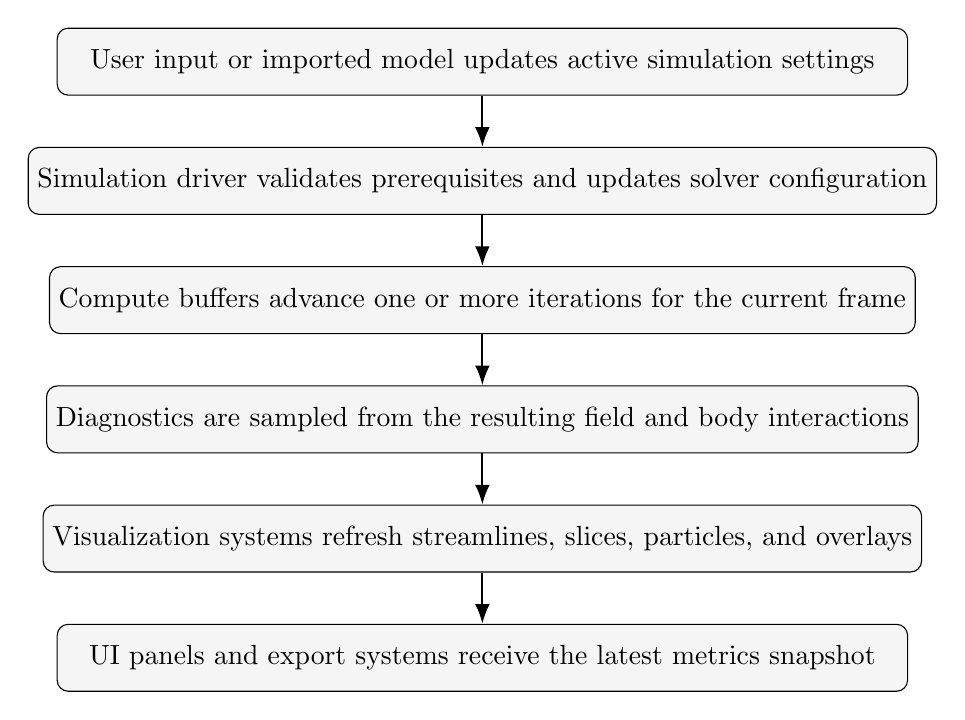
\begin{tikzpicture}[
node distance=0.65cm,
block/.style={draw, rounded corners, minimum width=10.8cm, minimum height=0.85cm, align=center, fill=gray!8},
arrow/.style={-{Latex[length=2.5mm]}, thick}
]
\node[block] (a) {User input or imported model updates active simulation settings};
\node[block, below=of a] (b) {Simulation driver validates prerequisites and updates solver configuration};
\node[block, below=of b] (c) {Compute buffers advance one or more iterations for the current frame};
\node[block, below=of c] (d) {Diagnostics are sampled from the resulting field and body interactions};
\node[block, below=of d] (e) {Visualization systems refresh streamlines, slices, particles, and overlays};
\node[block, below=of e] (f) {UI panels and export systems receive the latest metrics snapshot};
\draw[arrow] (a) -- (b);
\draw[arrow] (b) -- (c);
\draw[arrow] (c) -- (d);
\draw[arrow] (d) -- (e);
\draw[arrow] (e) -- (f);
\end{tikzpicture}
\caption{Frame-level data flow used by FluidWorks}
\label{fig:dataflow}
\end{figure}

\section{Architectural Rationale}
The architecture is intentionally modular because the project has to support different workflows without repeating the same control logic everywhere. The wind-tunnel path should be free to enforce its own rules, such as explicit flow-axis handling and vehicle reference-frame extraction, while internal flow should be free to require boundary assignment before the solve. A layered design prevents those requirements from becoming tangled together.

This same rationale explains why visualization is separated from the solver. Solver code can focus on field correctness and diagnostics, while the visualization layer can focus on legibility, mode-specific rendering, and scene behavior. That separation is a major reason the project can support both engineering-style outputs and presentation-friendly visuals in one application.

\chapter{Tools \& Technologies Used}
\section{Unity as the Runtime Platform}
Unity provides the project with a real-time scene graph, rendering pipeline, asset handling, input support, UI Toolkit, and compute-shader integration. For a project that combines engineering views with interactive model manipulation, Unity is a practical choice. It reduces the amount of custom engine work and lets the development effort stay focused on simulation logic and visualization quality.

\section{C\# Application Layer}
The high-level control code is written in C\#. This includes runtime model loading, scene orchestration, UI controllers, project persistence, metrics aggregation, and simulation drivers. C\# is also a good fit for repository organization because it keeps complex workflows readable and maintainable in an object-oriented structure.

\section{Compute Shaders}
The simulation core relies on compute shaders for field updates and parallel numeric work. This is especially important for the wind-tunnel solver and the free-surface implementation. Compute shaders allow the project to keep the update cycle on the GPU and preserve the responsiveness needed for interactive exploration.

\section{UI Toolkit}
Unity UI Toolkit is used to build the properties panels, analysis views, segmentation interface, and export controls. This is relevant to the report because a large part of the project value comes from how clearly the software exposes its controls and diagnostics. A readable interface is not separate from engineering usefulness; it is part of it.

\section{Runtime Geometry and Project Management}
The repository also contains runtime model import, part segmentation, project saving, and report-generation support. These are not secondary conveniences. They are necessary if the software is to be used repeatedly for classroom demonstrations, project reviews, or comparison studies on different models.

\section{Representative Technology Mapping}
\begin{table}[H]
\centering
\caption{Technology usage across major project areas}
\label{tab:techmap}
\begin{tabular}{p{3.2cm}p{4.0cm}p{5.8cm}}
\toprule
\textbf{Technology} & \textbf{Used In} & \textbf{Purpose} \\
\midrule
Unity Engine & Full application & Scene management, rendering, input, workflow integration \\
C\# & Runtime scripts & Simulation control, UI, metrics, project logic, export support \\
Compute Shaders & Wind tunnel, free surface & Parallel field updates and data-parallel numeric operations \\
UI Toolkit / UXML & Property panels and analysis views & Structured controls, diagnostics, and workflow-specific interfaces \\
CSV / JSON / HTML export & Reporting layer & Capture and communicate results outside the live runtime \\
Physics-informed MLP & Geometry analysis & Quick aerodynamic-quality prediction from extracted shape features \\
\bottomrule
\end{tabular}
\end{table}
